%Micah Chambers

\documentclass{beamer}
%\usepackage[orientation=landscape,size=custom,width=16,height=10,scale=0.5]{beamerposter} 

%\usepackage{pgfpages}
%\setbeameroption{show notes on second screen}

\mode<presentation>
{
  \usetheme{Antibes}
  % or ...

  %\setbeamercovered{transparent}
  % or whatever (possibly just delete it)
}

%\usefonttheme[onlylarge]{structurebold}
%\usecolortheme{crane}
%\setbeamerfont*{frametitle}{size=\normalsize,series=\bfseries}
%\setbeamertemplate{navigation symbols}{}
%\setbeamercovered{transparent}


\usepackage[pdftex]{graphicx}
\graphicspath{{pdf/}{png/}}
%\usepackage{times}
%\usepackage[T1]{fontenc}
%\usepackage[small]{caption}
\usepackage{algorithmic}

\title{Full Brain BOLD Signal Parameter Estimation \\
using Particle Filters}

%\subtitle{}

\author{Micah Chambers}
\institute{Virginia Tech Bioimaging Systems Lab}

\subject{Medical Imaging}

% If you have a file called "university-logo-filename.xxx", where xxx
% is a graphic format that can be processed by latex or pdflatex,
% resp., then you can add a logo as follows:

%\pgfdeclareimage[width=1.5cm]{university-logo}{logo}
\logo{
\includegraphics[width=1.5cm]{logo}}


% If you wish to uncover everything in a step-wise fashion, uncomment
% the following command: 

%\beamerdefaultoverlayspecification{<+->}


\begin{document}
\begin{frame}
  \titlepage
\end{frame}

\begin{frame}{Outline}
  \tableofcontents
  % You might wish to add the option [pausesections]
\end{frame}

\section{Introduction}
\begin{frame}{Balloon Model}
\begin{figure}
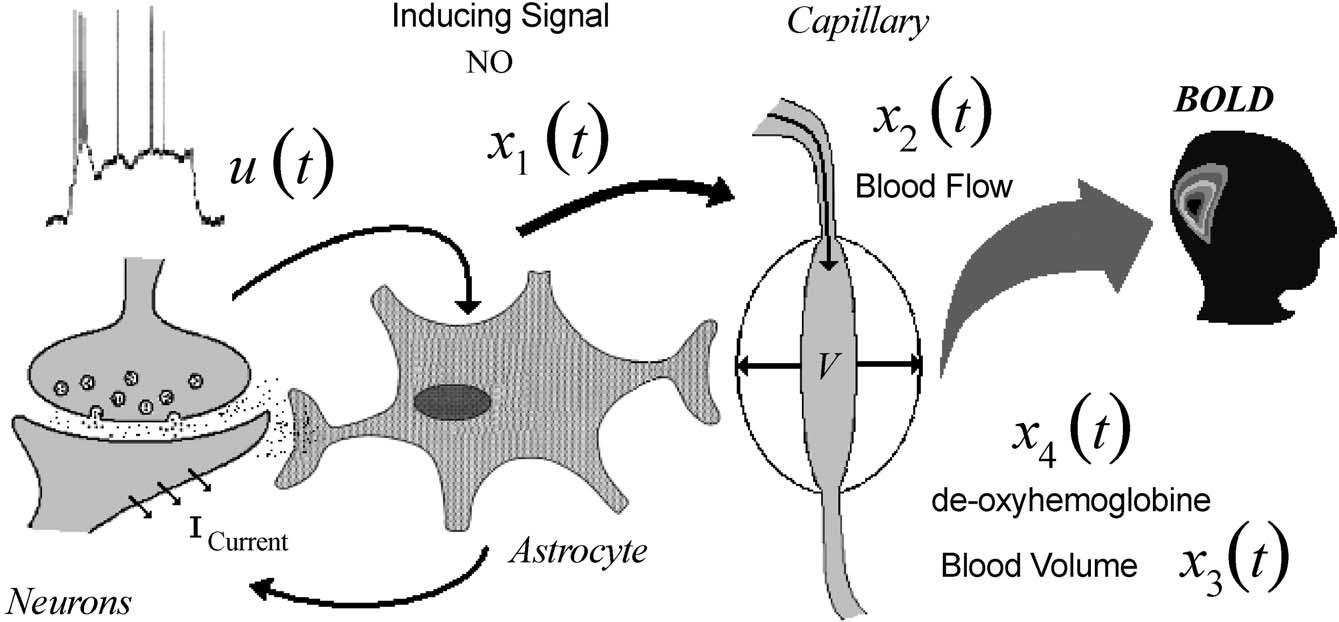
\includegraphics[width=10cm]{model}
\caption{
    \tiny
    \cite{Riera2003}
}
\end{figure}
\note{Rates range from below 1 Hz to 5 to 6 Hundred Hz}
\note{Change in average firing rates increase metabolism and sympathetic response causes
        increased inflow of oxygenated blood.}
\note{In the version of the Balloon model I used, the flow is locked to metabolism.}
\note{According the balloon model this increases the local blood volume, and the outflow pressure.}
\note{So the signal is altered by changes in the ratio of Deoxyhemoglobin and Oxygenated Hemoglobin,
        which are a function of Volume and Oxygenation.}
\end{frame}

\begin{frame}{Time Changing Parameters}
    \note{Should include a picture of the different parts of the BOLD signal}
\end{frame}

\begin{frame}{BOLD State Equations}
  \begin{itemize}
    \item Flow Inducing Signal
    $$\dot{s}(t) = \epsilon u(t) - s(t)/\tau_s - (f(t)/\tau_f - 1)$$
    \item Normalized Cerebral Blood Inflow:
    $$\dot{f}(t) = s $$
    \item Normalized Cerebral Blood Volume:
    $$\dot{v}(t) = (1/\tau_0)( f(t) - v(t) ^ {1/\alpha}) $$
    \item Normalized Deoxyhaemoglobin Content:\\
    $$\dot{q}(t) = \frac{1}{\tau_0}\left(\frac{f(t)(1-(1-E_0)^{1/f(t)})}{E_0} -
            \frac{q(t)}{v(t)^{1-1/\alpha}}\right)$$
    \item Hemodynamic Response - BOLD Signal
    $$y(t) = V_0(a_1( 1 - Q(t)) - a_2(1 - V(t)))$$
  \end{itemize}
  \note{System is dissipative:}
  \note{If no input is provided, it will rather quickly decay.}
  \note{Constant input leads to steady state response.}
  \note{First term in $\dot{q}$ is the metabolism term.}
  \note{Outflow is the $v^{1/\alpha}$ term}
  \note{Significant nonlinearity.}
\end{frame}

\section{Regression}
\begin{frame}{Approximate Method}
  \begin{itemize}
    \item 2nd Order Volterra Kernel \cite{Friston2000}
    \note{Quadratic Approximation}
    \begin{itemize}
        \item Quadratic Convolution used to approximate Jacobian Matrix.
        \note{Because of the nonlinearities in the BOLD model, step size for
                integrating would otherwise be extremely small}
        \item Volterra approximation quality is not known.
    \end{itemize}
    \note{Volterra Approximation depends on sparsity etc}
    {\footnotesize
    $$y(t) = k_0 + \int_{-\infty}^{\infty} k_1(s_1) x(t-s_1) ds_1
        + \int_{-\infty}^{\infty} k_2(s_1,s_2) x(t-s_1)x(t-s_2) ds_1 ds_2$$
        \note{Its possible this isn't even knowable}
    }
    \item Canonical Hemodynamic Response Function
    \note{Linear Approximation}
    \begin{itemize}
        \item No Parameters Estimated
        \item Maximum Likelihood Possible
        \item Inflexible - even to changes in onset time
    \end{itemize}
    \begin{center}
    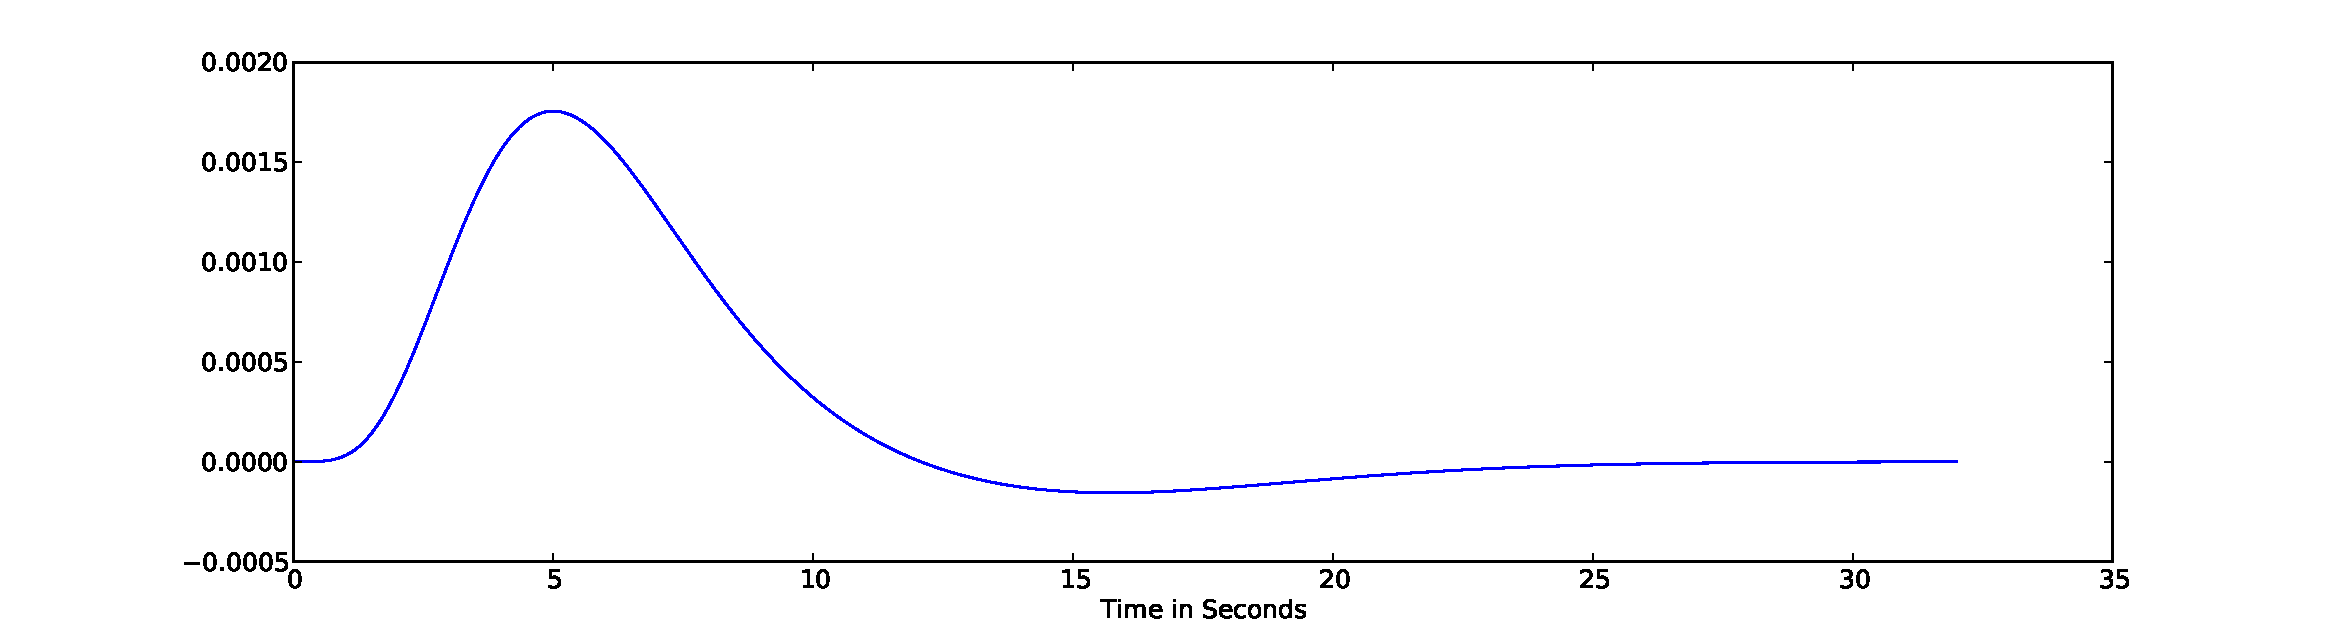
\includegraphics[clip=true,trim=4.88cm 0cm 5cm 1.5cm,height=2.7cm,width=8cm]{HRF}
    \end{center}
    
  \end{itemize}
\end{frame}

\begin{frame}{Nonlinear Modeling}
\begin{itemize}
    \item Local Linearization filter \cite{Riera2003}
     \note{Jacobian of the $\dot{x}$ is available, making gradient descent possible}
    \item Genetic Algorithms and Simulated Annealing \cite{Vakorin2007}
     \note{Genetic Algorithms were used to optimize spike points, simulated annealing for the parameters}
    \item Particle Filters to estimate $P(X_t | \Theta, Y_T)$ \cite{Murray2009}
    \begin{itemize}
        \item ML estimate of $\Theta$ based on $P(X_t | \Theta, Y_t)$ \cite{Johnston2007}
         \note{Particle Filter used to estimate states, ML of parameters based on the posterior of states and so on}
    \end{itemize}
    \item Unscented Kalman Filter to estimate parameters \cite{Hu2009}
    \item Direct Particle Filter, used in this work
     \note{Technically Kalman Filters and Particle Filters are Bayesian Filters}
     \note{Essentially filtering out inconsistent parameters.}
\end{itemize}
\end{frame}

\section{Particle Filter}
\begin{frame}{Construction}
\begin{itemize}
    \item Initialize Particles with Prior ($\alpha$):\\
        $$\{(x^i_0,w^i) : x^i_0 \sim \alpha(X), w^i = 
                \frac{1}{N_p}, i \in \{1, 2, ... , N_p\} \}$$
        $$\alpha(X) \stackrel{\text{\tiny{k=0}}}{\approx} P(x_k) 
                = \sum_{i=0}^{N_p} w^i\delta(x_k - x^i_k ) dx$$
    \item Particle Weights at time $t_k$:\\
        $$w^i_k \propto \frac{P(x^i_{0:k} | y_{0:k})}{q(x^i_{0:k} | y_{0:k})}$$
      \note{$q$ is the density/location of the particle}
      \note{$p$ is the actual probability }
    \item Adding Measurements:\\
        $$w^i_k \propto & w^i_{k-1}P(y_k| x_k) $$
      \note{Because of the proportion, note that the weights do not
            have to integrate to 1, and can be extremely large or extremely small}
\end{itemize}
\end{frame}

\begin{frame}{Details and Example}
  \begin{columns}
    \begin{column}{.55\textwidth}
        \begin{itemize}
            \item Non-parametric
            \item Model based
            \item Online
            \item Provides Full Posterior Probability
            \item Non-trivial computation cost
            \item Regularized Particle Filter Used
        \end{itemize}
    \end{column}
    \begin{column}{.45\textwidth}
        \begin{figure}
          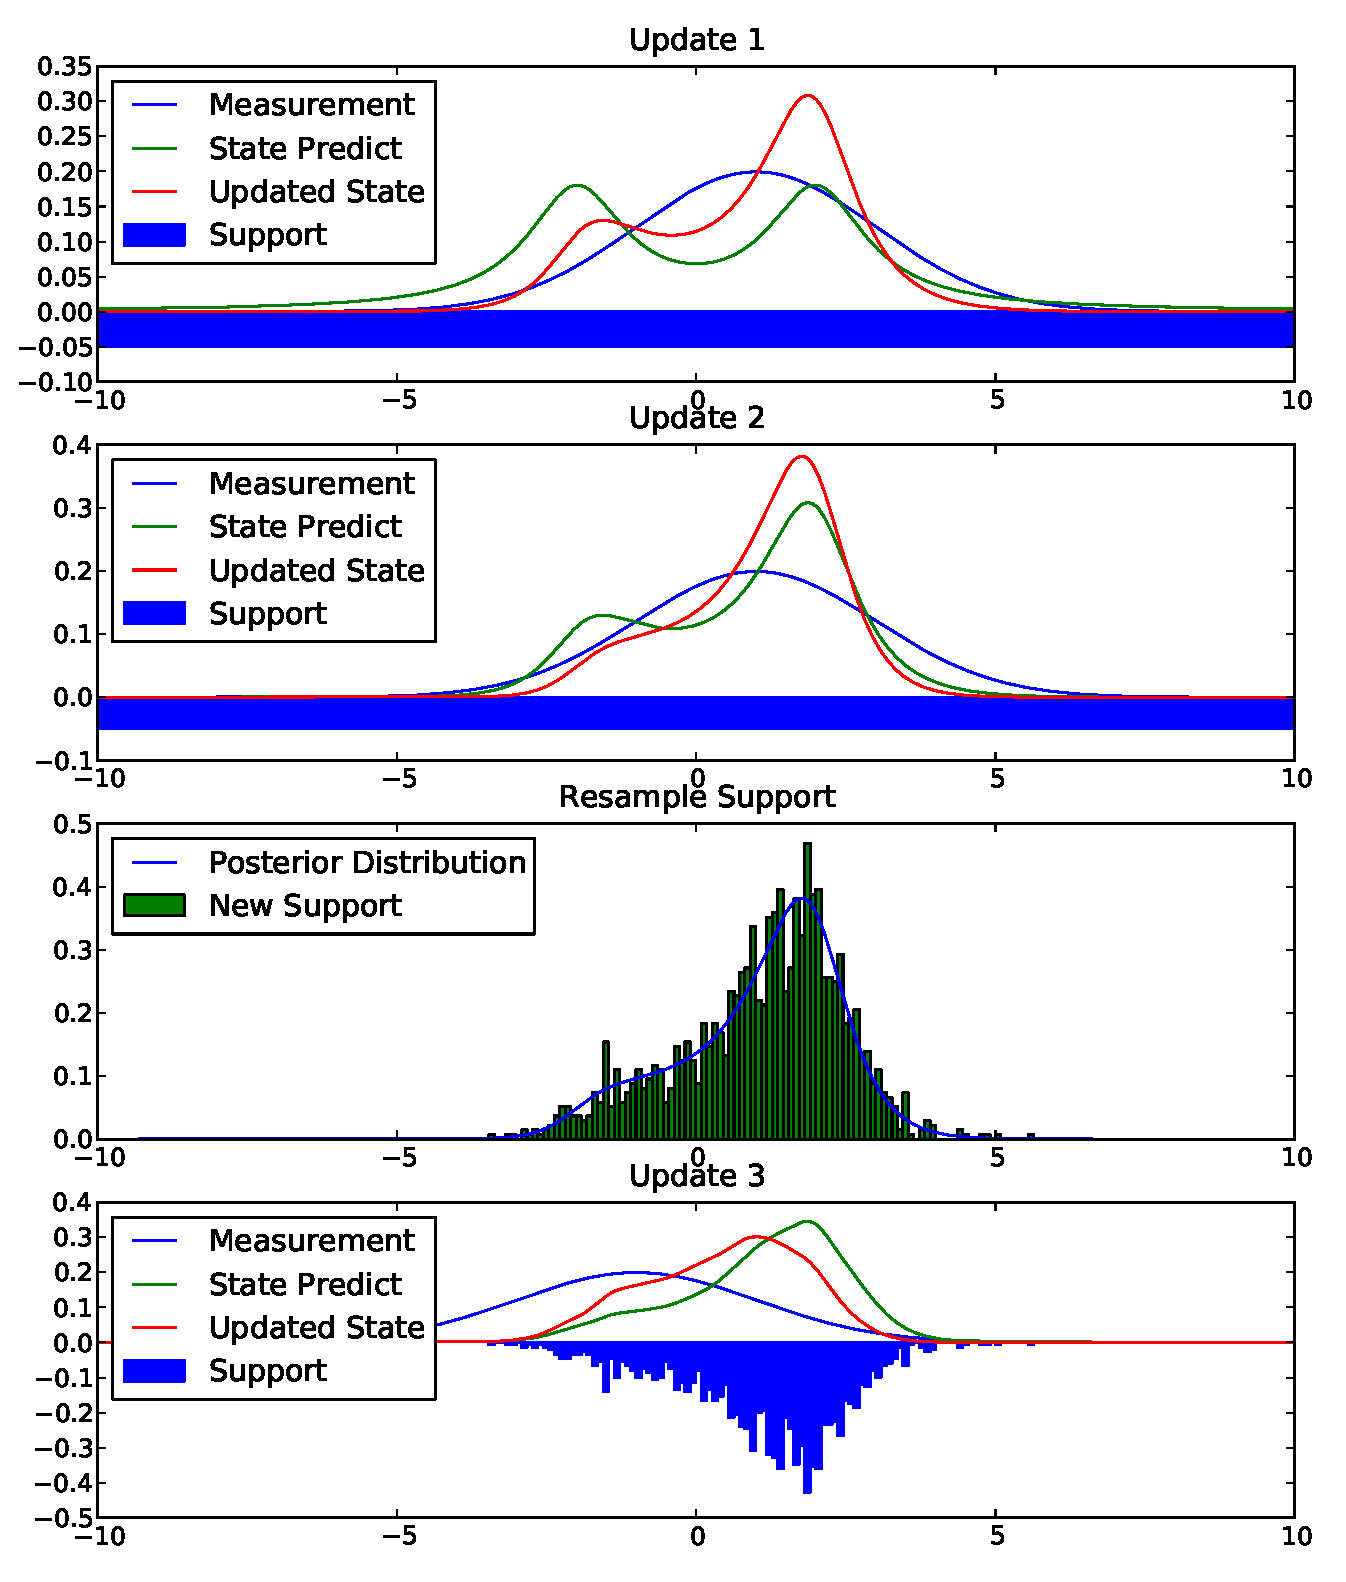
\includegraphics[width=\textwidth]{particle_filter}
        \end{figure}
    \end{column}
    \end{columns}
\end{frame}

%todo I should probably add labels on the axes
\section{Methods}
\begin{frame}{FMRI Noise}
\centering

Resting State Noise

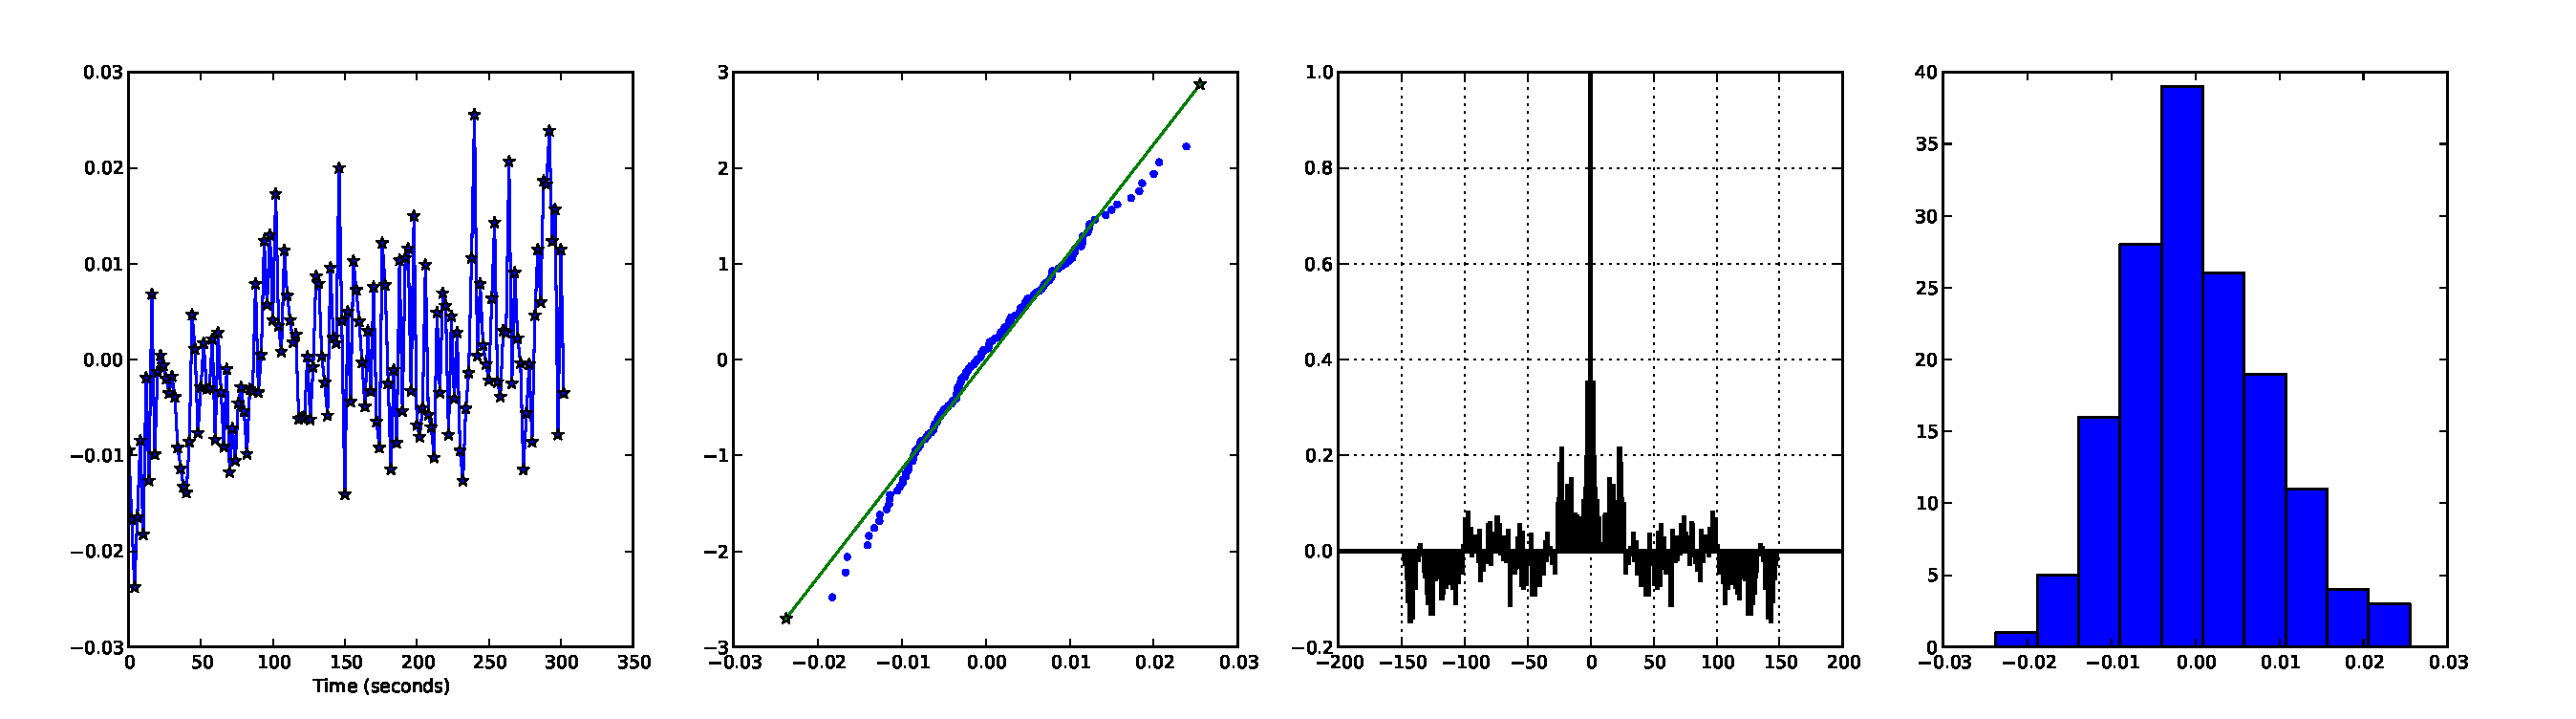
\includegraphics[trim=3cm 0cm 3cm 0cm,width=.75\textwidth]{noise2_0009_22_38_23}

Resting State Noise Steps

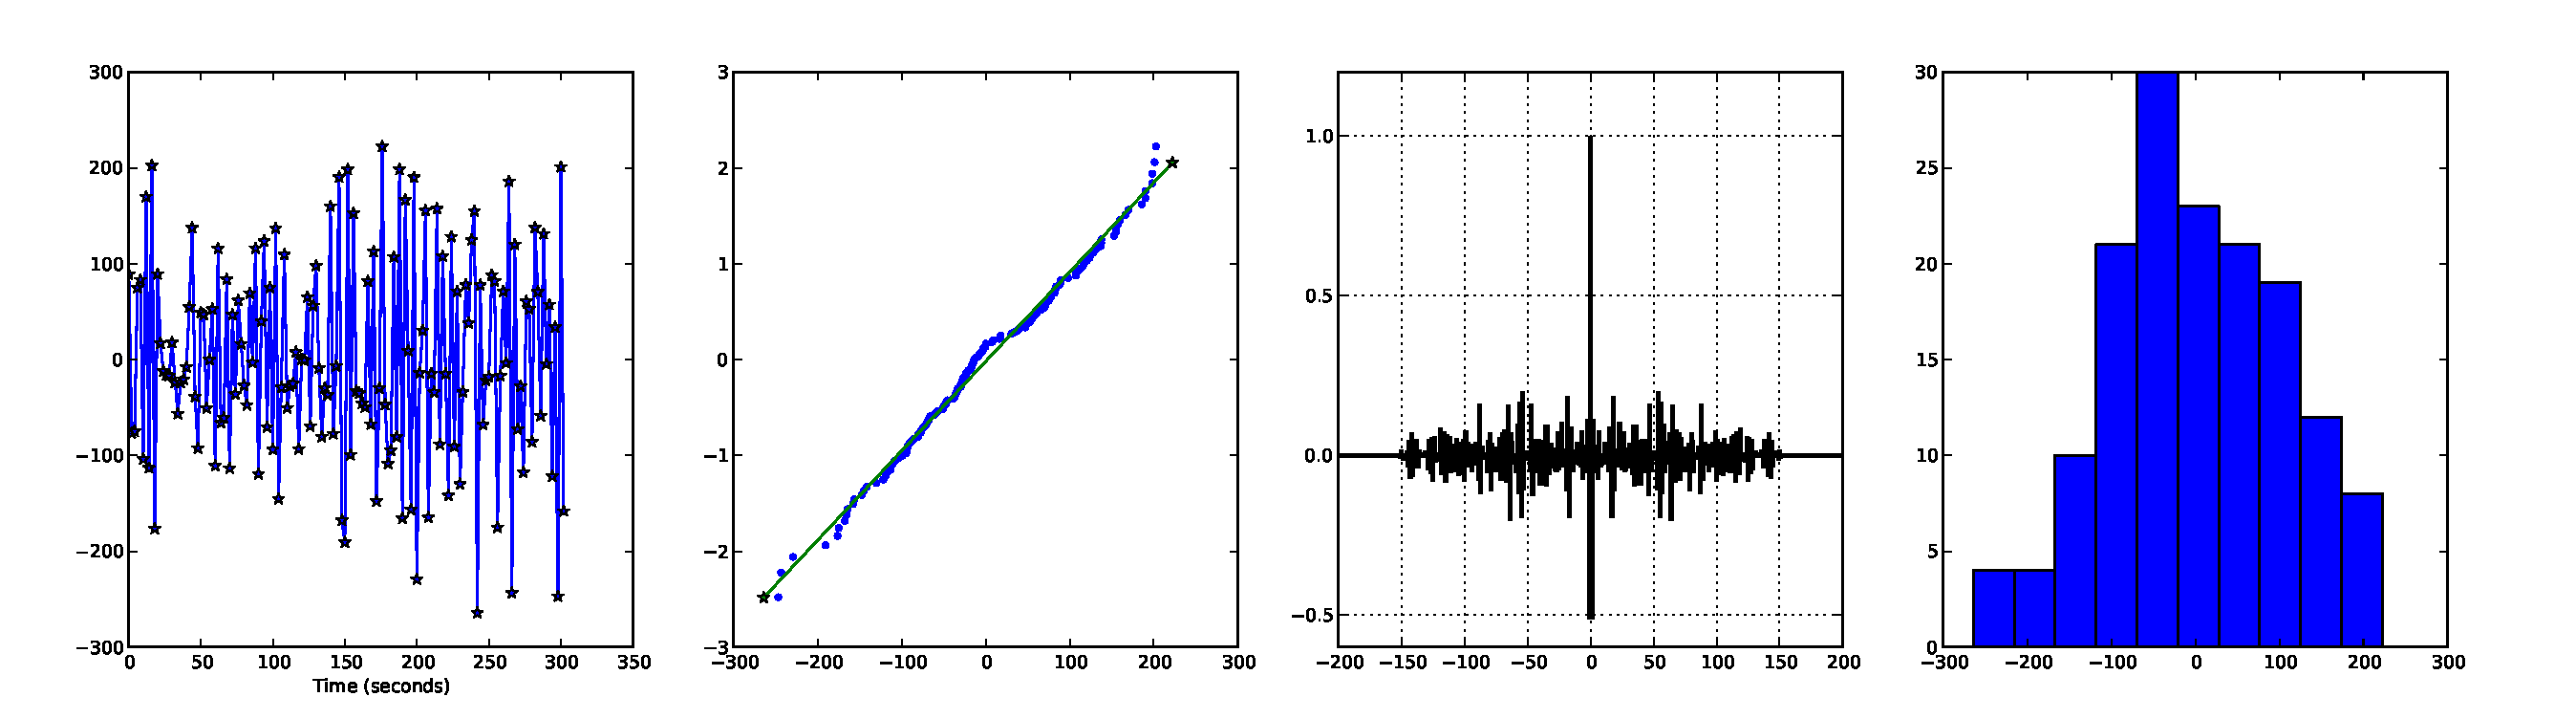
\includegraphics[trim=3cm 0cm 3cm 0cm,width=.75\textwidth]{noise2_0009d_22_38_23}

\note{Tanabe 2002 \autoref{Tanabe2002} 10-15\% of voxels exhibit significant drift}
\note{Occurs in Cadavers.}
\end{frame}

\begin{frame}{Preprocessing}
  \begin{columns}
    \begin{column}{.7\textwidth}
        \begin{itemize}
            \item Drop Inital Volumes (9 Here)
            \item Realign Over Time
            \item Detrend
            \item Gaussian Smoothing (SPM Only)
            \begin{itemize}
                \item Imposes Gaussianity
                \item Increases SNR
                \item Reduces Bonferroni Correction Requirement
            \end{itemize}
        \end{itemize}
    \end{column}
    
    \begin{column}{.3\textwidth}
    %todo graphic of preprocessing
    \end{column}
  \end{columns}
\end{frame}

\section{Results}
\begin{frame}{Long Run Results}
%convergence
%correlation
\end{frame}

\begin{frame}{Short Run Results}
%results image
%table of estimated parameters
\end{frame}

\begin{frame}{POSSUM Results}
%mutual information map
\end{frame}

\begin{frame}{SPM vs. Mutual Information Map}

\end{frame}

\begin{frame}{Factors Affecting Convergence}
    \begin{itemize}
        \item Weighting function
            \begin{itemize}
                \item Continuous, Long Tailed, Zero-Mean 
                \begin{itemize}
                \item Too wide -> under-sensitivity, slow or no convergence
                \item Too thin -> reduces robustness to noise, particle deprivation
                \end{itemize}
            \end{itemize}
        \item Resampling 
            \begin{itemize}
                \item Stratified Resampling can result in truncated tails 
                        on posterior
                \item Regularized Resampling can result in over smoothing and 
                        slow convergence
            \end{itemize}
        \item Number of particles
            \begin{itemize}
                \item More particles give higher fidelity posterior
            \end{itemize}
    \end{itemize}
\end{frame}

\section{Conclusion}
\begin{frame}{Key Findings}

\end{frame}

\begin{frame}{Conclusion}
\end{frame}

%% All of the following is optional and typically not needed. 
%\appendix
%\section<presentation>*{\appendixname}
%\subsection<presentation>*{For Further Reading}

\begin{frame}[allowframebreaks]
  \bibliographystyle{plain}
  \bibliography{../library}
\end{frame}

\end{document}



